\section{Scoping and symbol tables}
Scoping was implemented using a simple tree structure consisting of parent- and
child scopes. XQuery only allows new scopes to be defined through the
enclosedExpr production rule. This makes it trivial to start a new scope at the
beginning of a enclosedExpr, and end the scope and the end of an enclosedExpr.
This has been implemented as follows:
\begin{figure}[!h]
\begin{verbatim}
enclosedExpr : 
    LBRACESi {
        Scope parent = this.currentScope; 
        this.currentScope = new Scope(); 
        this.currentScope.setParent(parent); 
    }
    expr 
    RBRACSi { 
        this.currentScope = this.currentScope.getParent(); 
    }
;
\end{verbatim}
\caption{Scoping logic embedded in grammar definition}
\end{figure}

Where this.currentScope is a reference to the ``current'' scope in this
context. This member variable is initiated with an empty scope when an object
of the parser class is instantiated.

The implementation above (which is formatted slightly for brevity) will
automatically build a scope tree as the input is parsed.

The currentScope object, which is an object of type Scope, holds one reference
to a symbol table. The symbol table, which is a simple subclass of
java.util.HashMap, is not capable of performing symbol lookups throughout the
scope tree. This functionality is rather provided by the Scope class. The UML diagram
in figure \ref{fig:scope:uml1} illustrates the relationship between the Scope, SymTab, and Symbol
classes. \clearpage
\begin{figure}[!h]
  \centering
    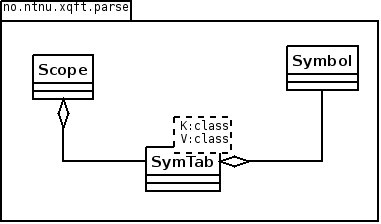
\includegraphics[scale=0.6]{img/uml1}
  \caption{Simplified UML overview of classes related to scope and symbol table}
  \label{fig:scope:uml1}
\end{figure}

\section{Type checking}
XQuery/XPath has a well-defined type hierarchy.
\begin{figure}[h!]
  \centering
    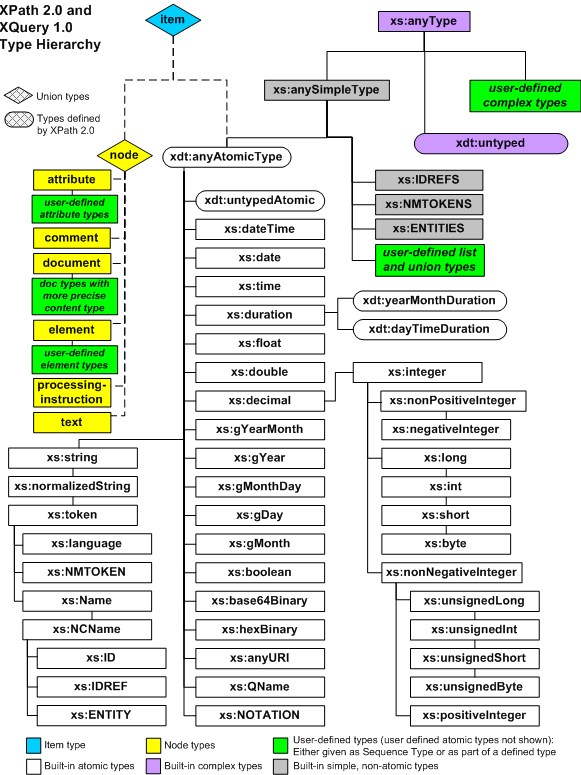
\includegraphics[scale=0.5]{img/xpathtypehierarchy}
  \caption{XQuery/XPath type hierarchy \cite{w3c04} (copyright
  \copyright W3C)}
\end{figure}
Here is a short overview of the basic type system:
\begin{itemize}
  \item Node types
    \begin{itemize}
      \item element()
      \item attribute()
      \item text()
      \item commment()
      \item document-node()
      \item processing-instruction()
    \end{itemize}
  \item Structure types
    \begin{itemize}
      \item Atomic types (xs:integer, xs:string, ..)
      \item Simple types (list, union)
      \item Complex types (user-defined types from an XML schema, except
      xs:anyType and xdt:untyped)
    \end{itemize}
\end{itemize}

Atomic types are strongly typed except xs:untypedAtomic, xs:anyURI, as well as
numerical types (xs:integer, xs:double, ..). Non-atomic simple types as well as
complex types are both strongly typed.

Proper type checking requires implementation of type inference and type
synthesis. This requires a stable abstract syntax tree and advanced data flow
analysis techniques to be feasible. Due to the inherent limitations in this
project, type checking has not been implemented - however the possibility of
this is discussed in section \ref{sect:summary:future_work}.

\underline{\textbf{\LARGE //TODO:}}
\begin{itemize}
  \item Dynamic vs. Static typing
  \item Strong vs. Weak (what and when)
  \item Type inference
  \item Michael Rys
\end{itemize}

\underline{\textbf{\LARGE //ODOT:}}